\documentclass{article}
\usepackage[utf8]{inputenc}
\usepackage[czech]{babel}
\usepackage[dvipsnames]{xcolor}

\usepackage{graphicx}
\usepackage{ulem,amsmath,bm}
\usepackage{amsmath}
\def\baselinestretch{1}\normalsize 
\usepackage{wrapfig}
\usepackage{pgf,tikz} 
\usepackage{dsfont}


\usepackage[bottom]{footmisc}
\usepackage{footnote}
\usepackage{textcomp}
\usepackage{amssymb}
\usepackage{url}
\usepackage{float}
\usepackage{caption}
\usepackage{subcaption}
\usepackage{multirow}
\usepackage[total={17cm,25cm}, top=3cm, left=2.5cm, right=2.5cm, bottom = 2cm, includefoot]{geometry}


\usepackage{braket}
\usepackage{mathtools}



\begin{document}
\begin{center}
    \Large
    \textbf{Poznámky}
           
    \vspace{0.4cm}
    \small
    \today
\end{center}

\section{Výpočet spektra}

Z (Iachello, Oss - Algebraic approach to molecular spectra: Two-dimensional problems) máme
$$\bra{N,n+1,l\pm1} \hat{D}_{\pm} \ket{N,n,l} = \pm \sqrt{n \pm l +2 }\sqrt{N - n},$$
kde výraz platí pro oba operátory $\hat{D}_{\pm}$ ($\pm$ nealternuje). Dále pracujeme s hamiltoniánem

$$\hat{H} = (1-\xi)\hat{n} -\frac{\xi}{N-1}\bigg[ \frac{1}{2}\left(\hat{D}_{+} \hat{D}_{-}+\hat{D}_{-} \hat{D}_{+}\right)+\hat{l}^{2}\bigg]
-\varepsilon\bigg[\frac{1}{2}(\hat{D}_+ + \hat{D}_-)\bigg].$$

Ten jsme sestavili ve dvou bázích $\ket{N,n,l}$ a $\ket{N,l,n}$

\begin{figure}[H]
    \centering
    \begin{subfigure}{.5\textwidth}
      \centering
      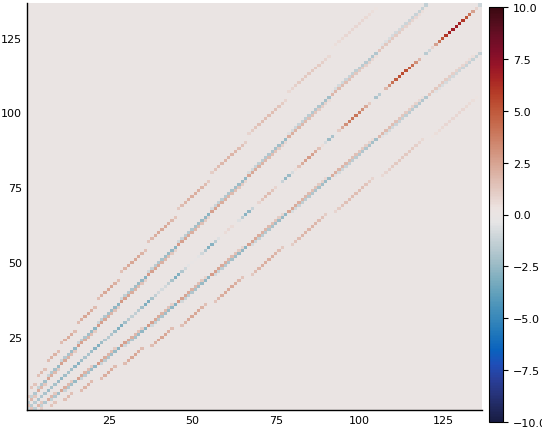
\includegraphics[width=.95\linewidth]{Nnl.png}
      \caption{$\ket{N,n,l}$}
      \label{fig:sub1}
    \end{subfigure}%
    \begin{subfigure}{.5\textwidth}
      \centering
      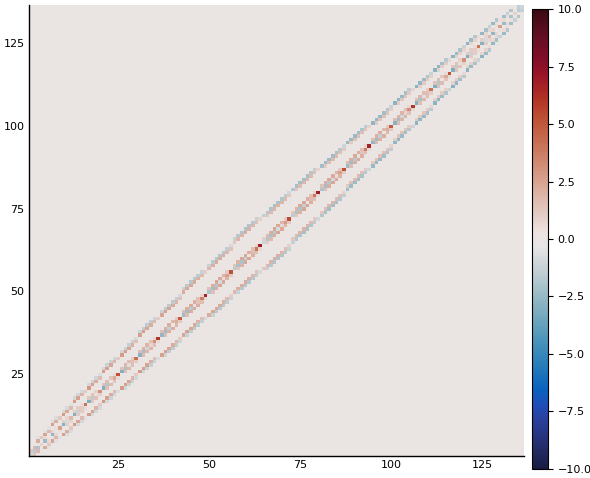
\includegraphics[width=.95\linewidth]{Nln.png}
      \caption{$\ket{N,l,n}$}
      \label{fig:sub2}
    \end{subfigure}
    \caption{Hamiltoniány ve dvou bázích}
    \label{fig:test}
    \end{figure}

\subsection{Diagonalizace}
\begin{itemize}
    \item \texttt{eigen()} - zatím nejrychlejší, ale neumí pracovat se sparse maticemi
    \item \texttt{eigs()} - z ArPack, umí sparse matice, ale řádově pomalejší
    \item \texttt{ArnoldiMethod} - Arnoldi,Krylov - zatím nejpomalejší, sparse matice
\end{itemize}


\begin{figure}[H]
    \centering
    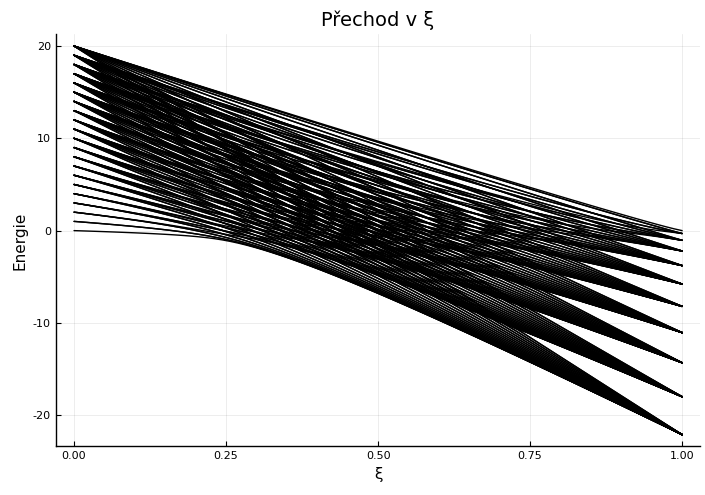
\includegraphics[width=.75\linewidth]{levels.png}
    \caption{Závislost hladin na $\xi$}
\end{figure}

\subsection{Úprava spektra}

\begin{itemize}
    \item \textcolor{red}{degenerace}
    \item polynomiální fit
    \item \textcolor{red}{cut}
    \item unfolding
    \item spacing
\end{itemize}

\begin{figure}[H]
    \centering
    \begin{subfigure}{.5\textwidth}
      \centering
      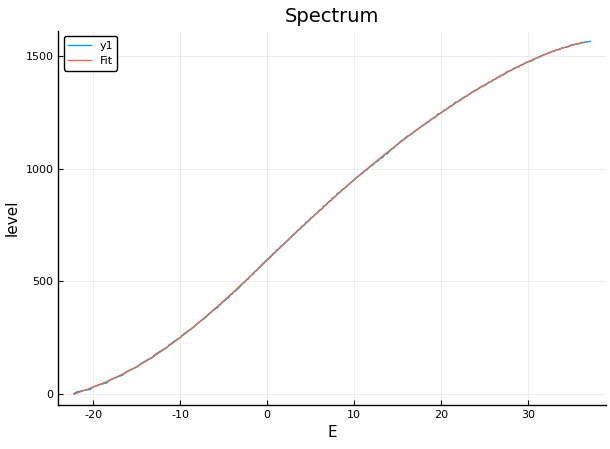
\includegraphics[width=.95\linewidth]{Fit.png}
      \caption{Fit}
      \label{fig:sub1}
    \end{subfigure}%
    \begin{subfigure}{.5\textwidth}
      \centering
      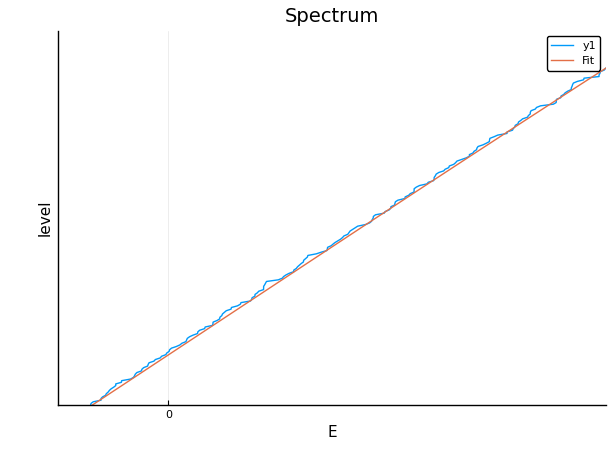
\includegraphics[width=.95\linewidth]{detail.png}
      \caption{Detail}
      \label{fig:sub2}
    \end{subfigure}
    \caption{Polynomiální fit spektra}
    \label{fig:test}
    \end{figure}


    \begin{figure}[H]
          \centering
          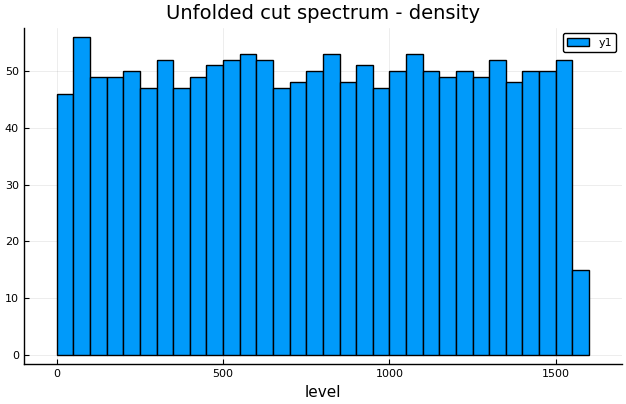
\includegraphics[width=.5\linewidth]{unfolded.png}
          \caption{Hustota hladin}
    \end{figure}



    \begin{figure}[H]
        \centering
        \begin{subfigure}{.5\textwidth}
          \centering
          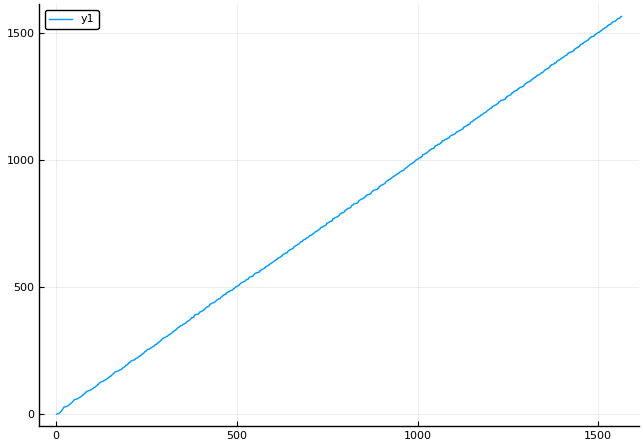
\includegraphics[width=.95\linewidth]{stretched.png}
          \caption{Natažení}
          \label{fig:sub1}
        \end{subfigure}%
        \begin{subfigure}{.5\textwidth}
          \centering
          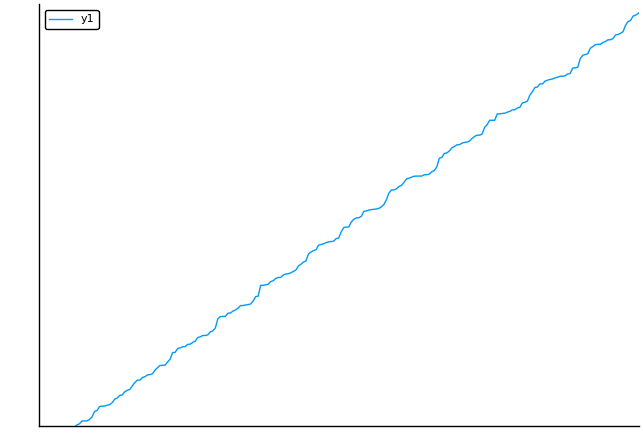
\includegraphics[width=.95\linewidth]{detailStretched.png}
          \caption{Detail}
          \label{fig:sub2}
        \end{subfigure}
        \caption{Natažení spektra}
        \label{fig:test}
        \end{figure}

\subsection{Indikátory chaosu}
\subsubsection{NNS - Brodyho parametr}
Brodyho parametr $\beta$ získáváme fitem spektra NNS 
$$P_{B}(s)=(\beta+1) b s^{\beta} e^{-b s^{\beta+1}}, \quad b=\left[\Gamma\left(\frac{\beta+2}{\beta+1}\right)\right]^{\beta+1}$$

$\beta \rightarrow 0$ je Poissonovo rozdělení (regulární) a $\beta \rightarrow 1$ je Wignerovo rozdělení (chaotické). 

\begin{figure}[H]
    \centering
    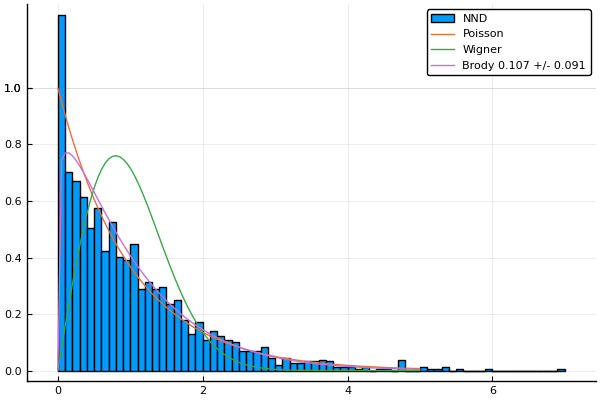
\includegraphics[width=.75\linewidth]{nns.png}
    \caption{Hustota hladin NNS s fitem}
  \end{figure}

  \begin{figure}[H]
    \centering
    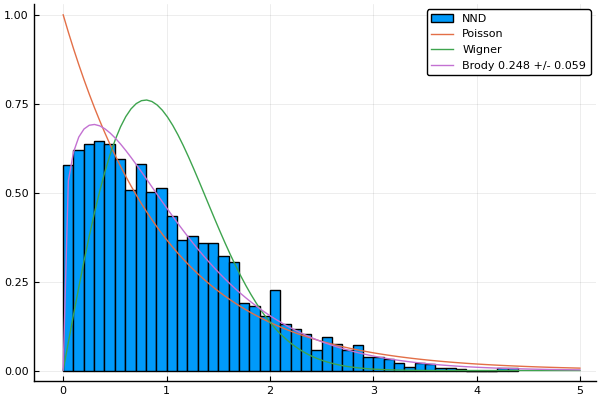
\includegraphics[width=.75\linewidth]{nns2.png}
    \caption{Hustota hladin NNS s fitem}
  \end{figure}

  \subsubsection{$\eta$}

  $$\eta \equiv \frac{\overline{\min (1 / r, r)}-I_{P}}{I_{\mathrm{WD}}-I_{P}}$$
  $r$ - podíl dvou nejbližších NNS bez unfoldingu
  \subsubsection{Delokalizace v bázi}
Vlastní stavy jsou vyjádřeny v bázi $\left\{\left|\phi_{j}\right\rangle\right\}_{j=0}^{D-1}$
jako $\left|\psi_{i}\right\rangle=\sum a_{i j}\left|\phi_{j}\right\rangle$. Definujeme
  $$\xi_{E}(i)=\left(\sum_{j=0}^{D-1}\left|a_{i j}\right|^{4}\right)^{-1}$$
  $$\bar{\xi}_{E}=\frac{1}{D \xi_{E}^{\mathrm{deloc}}} \sum_{i=0}^{D-1} \xi_{E}(i),$$
  kde $\xi_{E}^{\mathrm{deloc}} \approx Dim/3$.

  \begin{figure}[H]
    \centering
    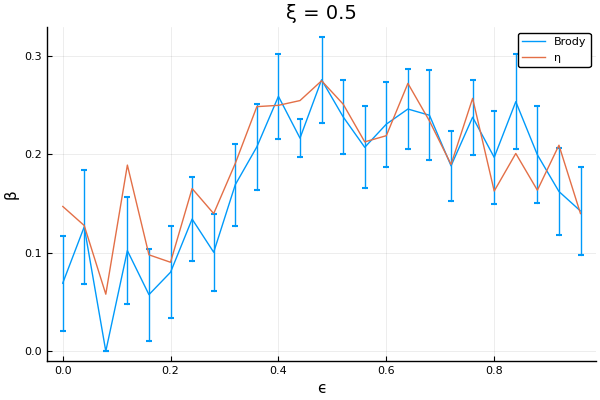
\includegraphics[width=.75\linewidth]{indicators.png}
    \caption{Indikátory chaosu - bez degenerace}
\end{figure}

    \begin{figure}[H]
        \centering
        \includegraphics[width=.75\linewidth]{indicators2.png}
        \caption{Indikátory chaosu - s degeneraci}
  \end{figure}

\end{document}
